\documentclass[journal]{IEEEtran}
\usepackage[utf8]{inputenc}
\usepackage[T1]{fontenc}
\usepackage[portuguese]{babel}
\usepackage{graphicx}
\usepackage{cite}
\usepackage{hyperref}
\usepackage{amsmath}
\usepackage{amssymb}
\usepackage{booktabs}
\usepackage{array}
\usepackage{microtype}
\graphicspath{{figures/}}
\hypersetup{colorlinks=true,linkcolor=black,citecolor=black,urlcolor=black}

\title{GraphQL vs REST em um Experimento Controlado:\\
Tempo de Resposta, Tamanho de Payload e Significância Estatística}

\author{Amanda Bueno Campos Peixoto\\
Guilherme Gomes de Brites\\
Lucas Cerqueira Azevedo\\[0.35em]
\small Laboratório de Experimentação de Software -- Lab 05}

\date{\today}

\begin{document}

\maketitle

\begin{abstract}
Este artigo relata um experimento controlado que compara REST e GraphQL sobre a mesma base SQLite, a mesma camada de serviços e cinco cenários de consulta. A coleta atualmente disponível contém 5.000 medições válidas, organizadas em 500 repetições pareadas por cenário e tecnologia. A análise avalia tempo de resposta e tamanho do payload por meio de estatísticas descritivas, testes pareados, correção de Holm e tamanho de efeito. Os resultados indicam vantagem clara de GraphQL em cenários com dados aninhados e redução consistente de payload em quatro dos cinco cenários, enquanto consultas simples apresentam diferenças temporais pequenas e não significativas.
\end{abstract}

\section{Introdução}
\label{sec:intro}

APIs REST continuam sendo uma escolha dominante para sistemas Web por sua simplicidade operacional e compatibilidade com HTTP. GraphQL propõe uma alternativa orientada a consulta, na qual o cliente especifica exatamente os campos desejados e pode recuperar estruturas aninhadas em uma única chamada. Essa flexibilidade promete reduzir over-fetching, under-fetching e múltiplas idas à rede, mas também pode introduzir custo de parsing e resolução no servidor.

O objetivo deste trabalho é comparar empiricamente REST e GraphQL em um ambiente controlado. O estudo mede duas dimensões observáveis pelo cliente: tempo total de resposta e tamanho do corpo retornado. A pergunta central é se GraphQL apresenta vantagem mensurável em relação a REST quando ambas as abordagens executam tarefas equivalentes sobre os mesmos dados.

\section{Metodologia}
\label{sec:methodology}

\subsection{Ambiente Experimental}

O experimento usa uma API Python local com endpoints REST e um endpoint GraphQL. As duas tecnologias compartilham o mesmo banco SQLite e a mesma camada de serviços, reduzindo diferenças de implementação que poderiam favorecer artificialmente uma abordagem. A base sintética padrão contém 1.000 usuários, 10.000 postagens e 50.000 comentários, gerados de forma determinística.

Os cenários avaliados foram: full profile, nested data, post titles, simple user, user list. Cada cenário foi executado nas versões REST e GraphQL. Nos cenários REST que exigem múltiplas chamadas, o tempo e o tamanho foram acumulados até completar a tarefa experimental, preservando equivalência funcional com a consulta GraphQL.

\subsection{Coleta}

A configuração usada nos dados atuais executou 10 chamadas de aquecimento por cenário e tecnologia, seguidas por 500 repetições válidas pareadas. Em cada repetição, a ordem entre REST e GraphQL foi randomizada para reduzir viés de aquecimento, cache e flutuação temporal. O dataset resultante possui 5.000 linhas válidas, exatamente 5 cenários $\times$ 2 tecnologias $\times$ 500 repetições.

A configuração padrão do coletor foi definida em 500 repetições por cenário, o que gera 5.000 medições válidas em uma nova execução completa. A razão é prática: 5.000 medições são suficientes para revelar grandes efeitos, mas os cenários simples apresentam diferenças temporais próximas do ruído de medição local. Manter esse volume de repetições melhora a precisão desses casos marginais sem alterar o desenho experimental.

\subsection{Análise Estatística}

Para cada cenário e métrica, as medições foram pareadas por repetição. A diferença foi definida como REST menos GraphQL; portanto, valores positivos indicam menor tempo ou payload em GraphQL. A normalidade das diferenças foi avaliada por Shapiro-Wilk. Quando a distribuição foi compatível com normalidade, aplicou-se teste t pareado; caso contrário, aplicou-se Wilcoxon pareado. Os p-valores foram corrigidos por Holm separadamente por métrica, com $\alpha = 0{,}05$.

\section{Resultados}
\label{sec:results}

\subsection{Visão Geral dos Efeitos}

\begin{figure}[!t]
\centering
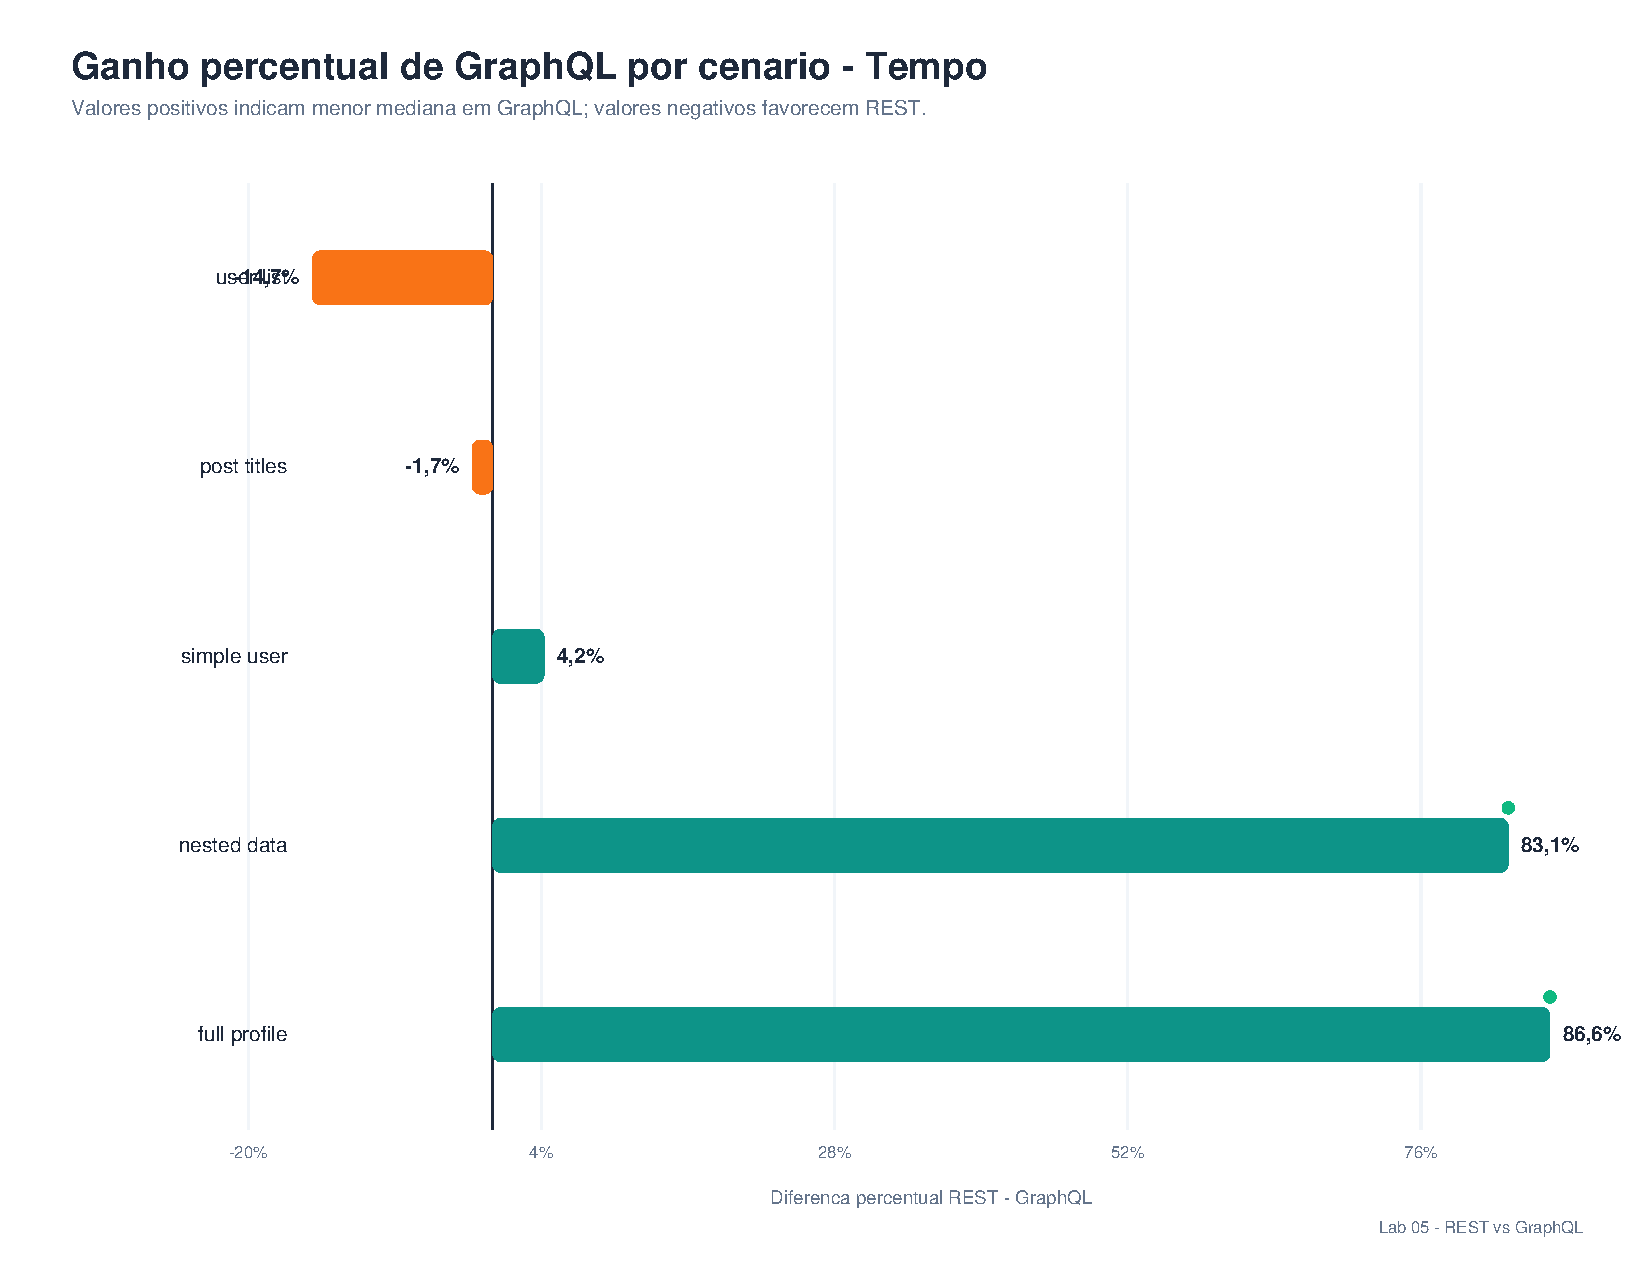
\includegraphics[width=\columnwidth]{time_gain.pdf}
\caption{Ganho percentual de GraphQL em tempo de resposta. Valores positivos indicam menor mediana em GraphQL.}
\label{fig:time_gain}
\end{figure}

A Figura \ref{fig:time_gain} mostra que GraphQL reduziu fortemente o tempo nos cenários \textit{nested data} e \textit{full profile}, com ganhos entre 83,1\% e 86,6\%. Esses cenários exigem múltiplas chamadas REST para recompor dados aninhados, enquanto GraphQL resolve a tarefa em uma consulta. Em contraste, consultas simples ficaram próximas da paridade, com diferenças entre -14,7\% e 4,2\%, e sem significância em 3 dos cinco testes temporais.

\begin{figure}[!t]
\centering
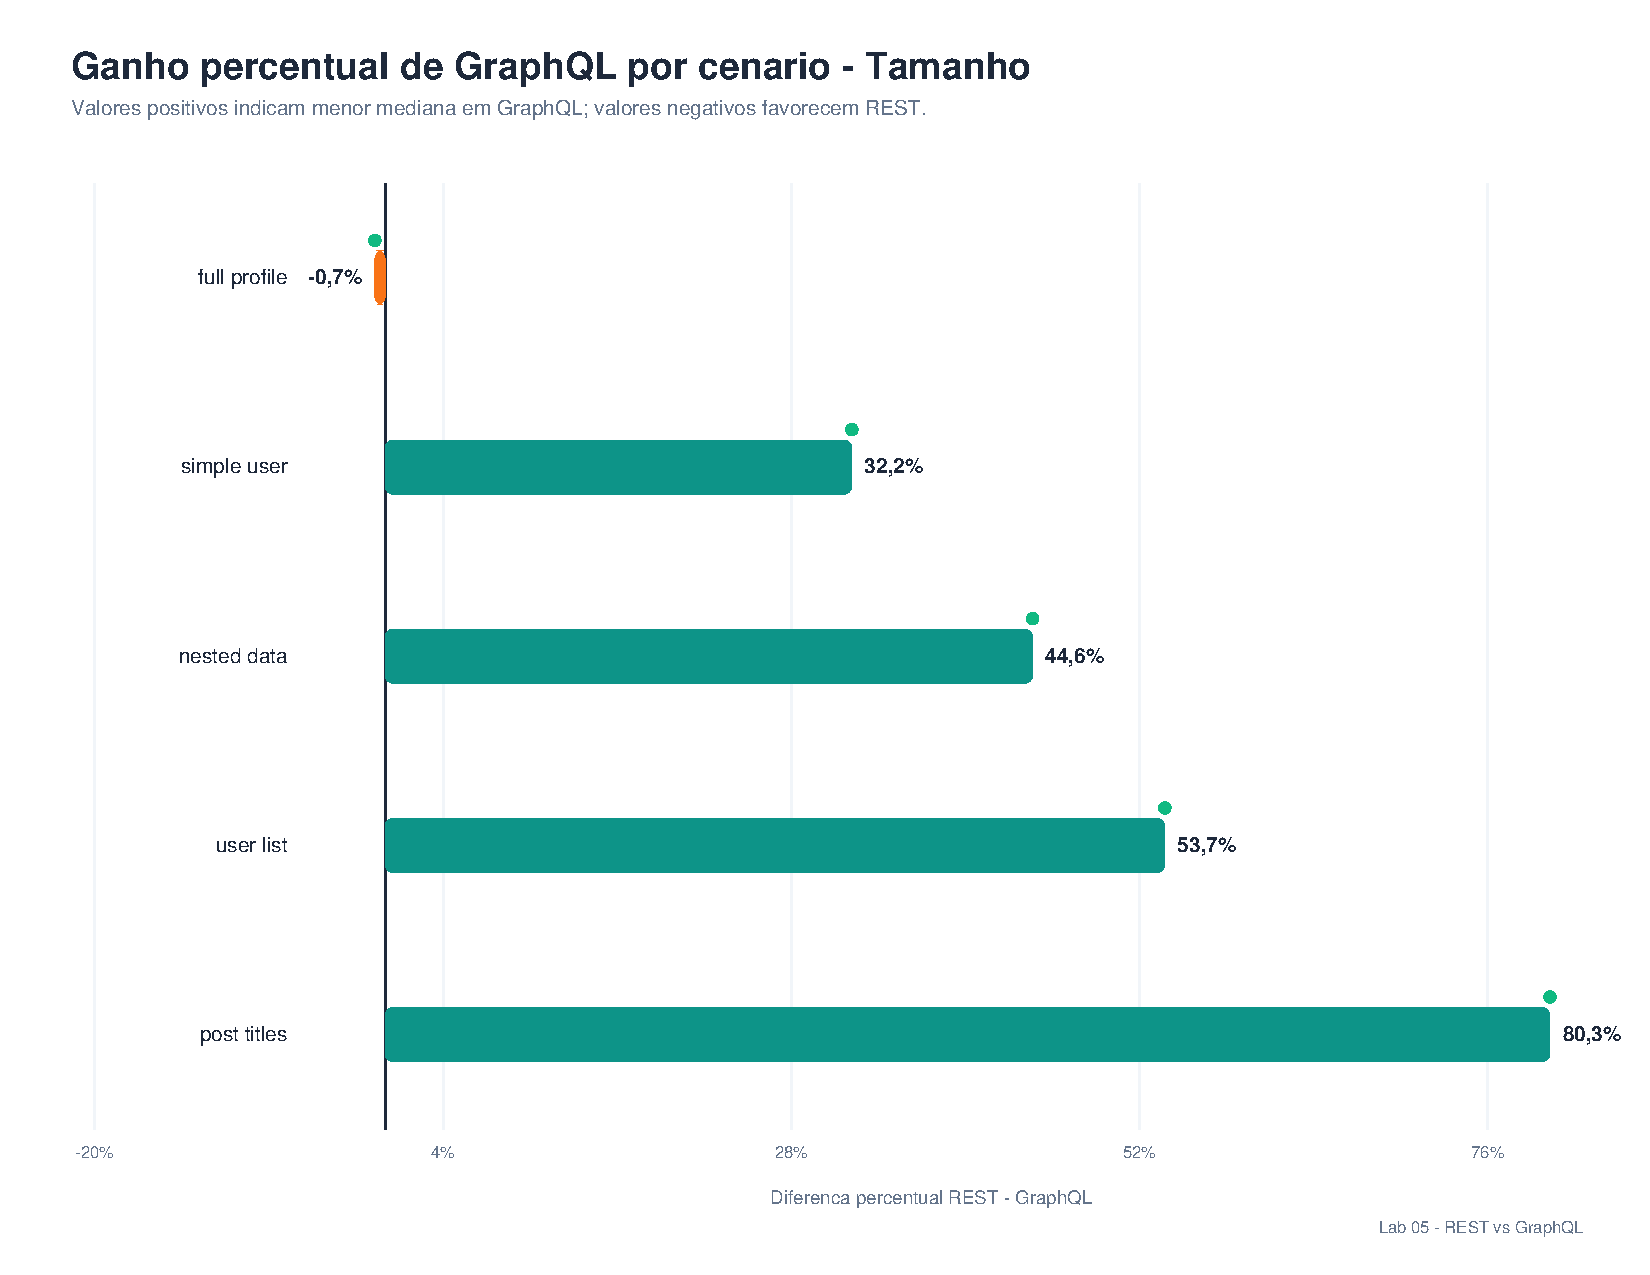
\includegraphics[width=\columnwidth]{size_gain.pdf}
\caption{Ganho percentual de GraphQL no tamanho da resposta. Valores positivos indicam menor payload em GraphQL.}
\label{fig:size_gain}
\end{figure}

A Figura \ref{fig:size_gain} evidencia uma vantagem mais consistente em tamanho de resposta. GraphQL reduziu o payload em 4 dos cinco cenários, com ganhos entre -0,7\% e 80,3\%. O único caso negativo foi \textit{full profile}, no qual a consulta GraphQL retornou uma representação praticamente equivalente à REST e ficou 0,7\% maior.

\subsection{Perfil Multivariado}

\begin{figure}[!t]
\centering
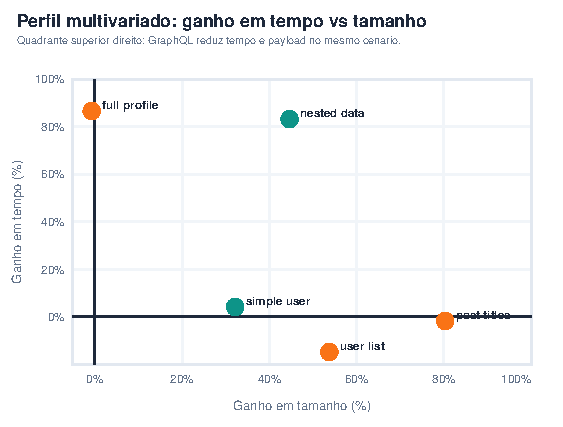
\includegraphics[width=\columnwidth]{quadrant_profile.pdf}
\caption{Perfil multivariado dos cenários: ganho em tamanho versus ganho em tempo.}
\label{fig:quadrant}
\end{figure}

A Figura \ref{fig:quadrant} combina as duas métricas. Os cenários aninhados aparecem no quadrante favorável a GraphQL em tempo e, em geral, também em tamanho. O cenário \textit{post titles} demonstra o caso clássico de redução de over-fetching: o tempo fica próximo da paridade, mas o payload cai substancialmente porque a consulta GraphQL solicita apenas títulos.

\subsection{Distribuição Temporal}

\begin{figure}[!t]
\centering
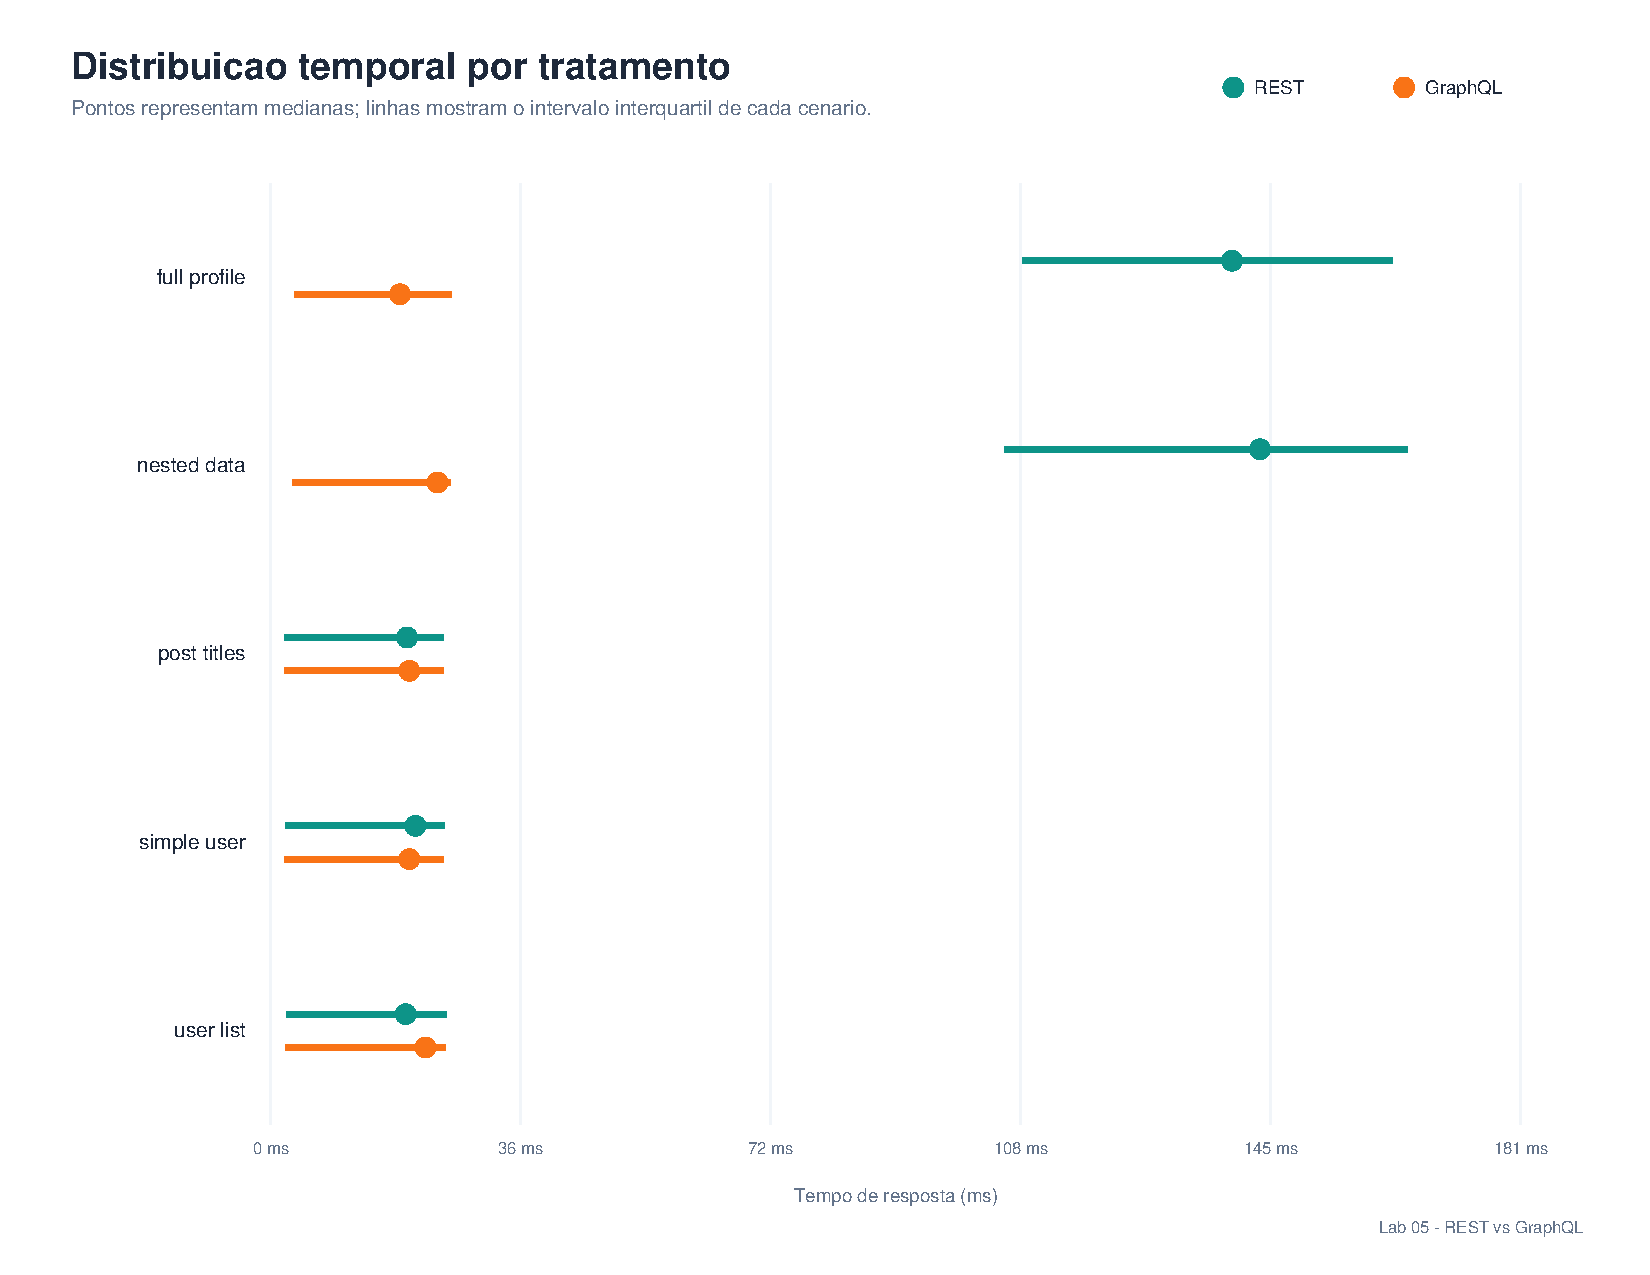
\includegraphics[width=\columnwidth]{time_intervals.pdf}
\caption{Medianas e intervalos interquartis do tempo de resposta por tratamento.}
\label{fig:time_intervals}
\end{figure}

A Figura \ref{fig:time_intervals} mostra que as distribuições de tempo dos cenários simples se sobrepõem mais do que as dos cenários aninhados. Isso explica a decisão estatística: quando a diferença é pequena diante da variabilidade local, a conclusão apropriada é paridade ou inconclusão, não vitória prática de uma tecnologia.

\subsection{Decisão Estatística}

\begin{figure}[!t]
\centering
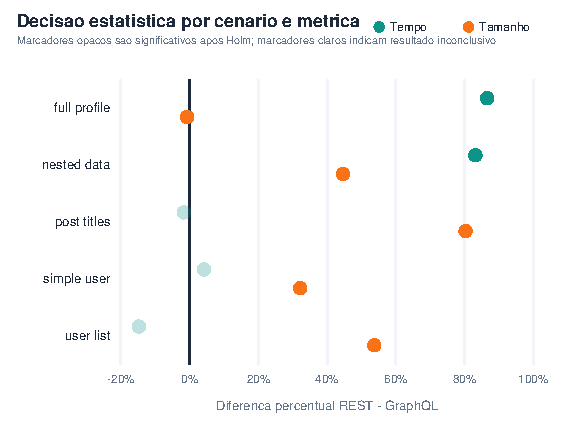
\includegraphics[width=\columnwidth]{statistical_decision.pdf}
\caption{Decisão estatística por cenário e métrica. Marcadores opacos indicam significância após correção de Holm.}
\label{fig:decision}
\end{figure}

A Figura \ref{fig:decision} resume os 10 testes pareados. Ao todo, 7 foram significativos. Para tempo de resposta, 2 de cinco cenários apresentaram diferença significativa. Para tamanho do payload, 5 de cinco cenários foram significativos, o que era esperado porque os tamanhos são determinísticos para uma mesma consulta e base de dados.

\begin{table*}[!t]
\centering
\caption{Resumo dos testes pareados. Dif. é REST menos GraphQL; valores positivos favorecem GraphQL.}
\label{tab:tests}
\footnotesize
\setlength{\tabcolsep}{6pt}
\renewcommand{\arraystretch}{1.12}
\begin{tabular}{llrrrrr}
\toprule
Cenário & Métrica & REST & GraphQL & Dif. & p Holm & Sig. \\
\midrule
        full profile & Tamanho & 5.608,00 & 5.647,00 & -0,7\% & 0,0000 & Sim \\
        full profile & Tempo & 138,96 & 18,68 & 86,6\% & 0,0000 & Sim \\
        nested data & Tamanho & 5.608,00 & 3.105,00 & 44,6\% & 0,0000 & Sim \\
        nested data & Tempo & 143,01 & 24,11 & 83,1\% & 0,0000 & Sim \\
        post titles & Tamanho & 1.359,00 & 268,00 & 80,3\% & 0,0000 & Sim \\
        post titles & Tempo & 19,70 & 20,02 & -1,7\% & 1,0000 & Nao \\
        simple user & Tamanho & 115,00 & 78,00 & 32,2\% & 0,0000 & Sim \\
        simple user & Tempo & 20,90 & 20,02 & 4,2\% & 1,0000 & Nao \\
        user list & Tamanho & 5.471,00 & 2.531,00 & 53,7\% & 0,0000 & Sim \\
        user list & Tempo & 19,50 & 22,37 & -14,7\% & 0,7968 & Nao \\
\bottomrule
\end{tabular}
\end{table*}

\section{Discussão}
\label{sec:discussion}

Os resultados sugerem que a vantagem de GraphQL depende do formato da tarefa. Quando a consulta exige dados aninhados ou seleção fina de campos, GraphQL reduz chamadas ou payload e tende a apresentar ganhos relevantes. Quando a tarefa já é simples em REST, como buscar um usuário ou listar usuários com poucos campos, o custo e o benefício ficam próximos da paridade.

O tamanho da resposta apresentou comportamento mais estável que o tempo, pois é determinado pelo formato do payload. O tempo de resposta, por outro lado, sofre influência de ruído local, escalonamento do sistema operacional e pequenas variações do servidor. A maior incerteza foi observada em user list, com erro padrão da diferença temporal de aproximadamente 2,00 ms. Por isso, o projeto recomenda manter pelo menos 500 repetições por cenário em novas coletas.

\section{Ameaças à Validade}
\label{sec:threats}

O estudo usa uma API local e uma base sintética; portanto, os resultados não devem ser generalizados diretamente para sistemas distribuídos, redes reais ou bancos sob carga concorrente. A implementação GraphQL e REST foi construída para equivalência funcional, mas bibliotecas e otimizações específicas poderiam alterar os resultados. Além disso, o tamanho de resposta mede apenas o corpo retornado, não cabeçalhos HTTP ou compressão. Finalmente, o experimento atual mede um único perfil de dados e parâmetros fixos de página, usuário e limite.

\section{Conclusão}
\label{sec:conclusion}

Neste experimento controlado, GraphQL apresentou ganhos expressivos nos cenários em que REST precisou realizar múltiplas chamadas ou retornou campos desnecessários. A vantagem mais clara ocorreu em \textit{full profile}, com 86,6\% de redução na mediana de tempo, e em \textit{post titles}, com 80,3\% de redução no tamanho da resposta. Para consultas simples, a evidência não sustenta uma superioridade temporal robusta. Assim, a conclusão principal é contextual: GraphQL se destaca quando a consulta precisa compor dados ou controlar seletivamente campos, enquanto REST permanece competitivo em endpoints simples e bem ajustados.

\begin{thebibliography}{99}

\bibitem{graphql} GraphQL Foundation, ``GraphQL Specification'', \url{https://spec.graphql.org/}.

\bibitem{fielding} R. T. Fielding, ``Architectural Styles and the Design of Network-based Software Architectures'', Doctoral dissertation, University of California, Irvine, 2000.

\bibitem{holm} S. Holm, ``A Simple Sequentially Rejective Multiple Test Procedure'', Scandinavian Journal of Statistics, 1979.

\bibitem{wilcoxon} F. Wilcoxon, ``Individual Comparisons by Ranking Methods'', Biometrics Bulletin, 1945.

\end{thebibliography}

\end{document}
